\chapter{Data and code availability}
In order to streamline my processes and make them more appealing to the public and to mitigate the risk of de-anonymization \cite{Nar08DeAnon}, a part of the agreement was not to publish any keystroke data of my testing subjects. At GitHub I have published the source code of \href{https://github.com/goalon/time-tracking}{my plugin}, the source code available for \href{https://github.com/goalon/time-tracking-analysis}{data analysis} and the Latex source code of \href{https://github.com/goalon/masters-thesis}{this thesis}. Anyone also can download my plugin directly from VS Code or at \href{https://marketplace.visualstudio.com/items?itemName=MateuszBajorekMIMUW.mimuw-mb-tt-time-tracking}{Visual Studio Marketplace} \ref{fig:marketplace}.

\begin{figure}[htbp]
  \centering
  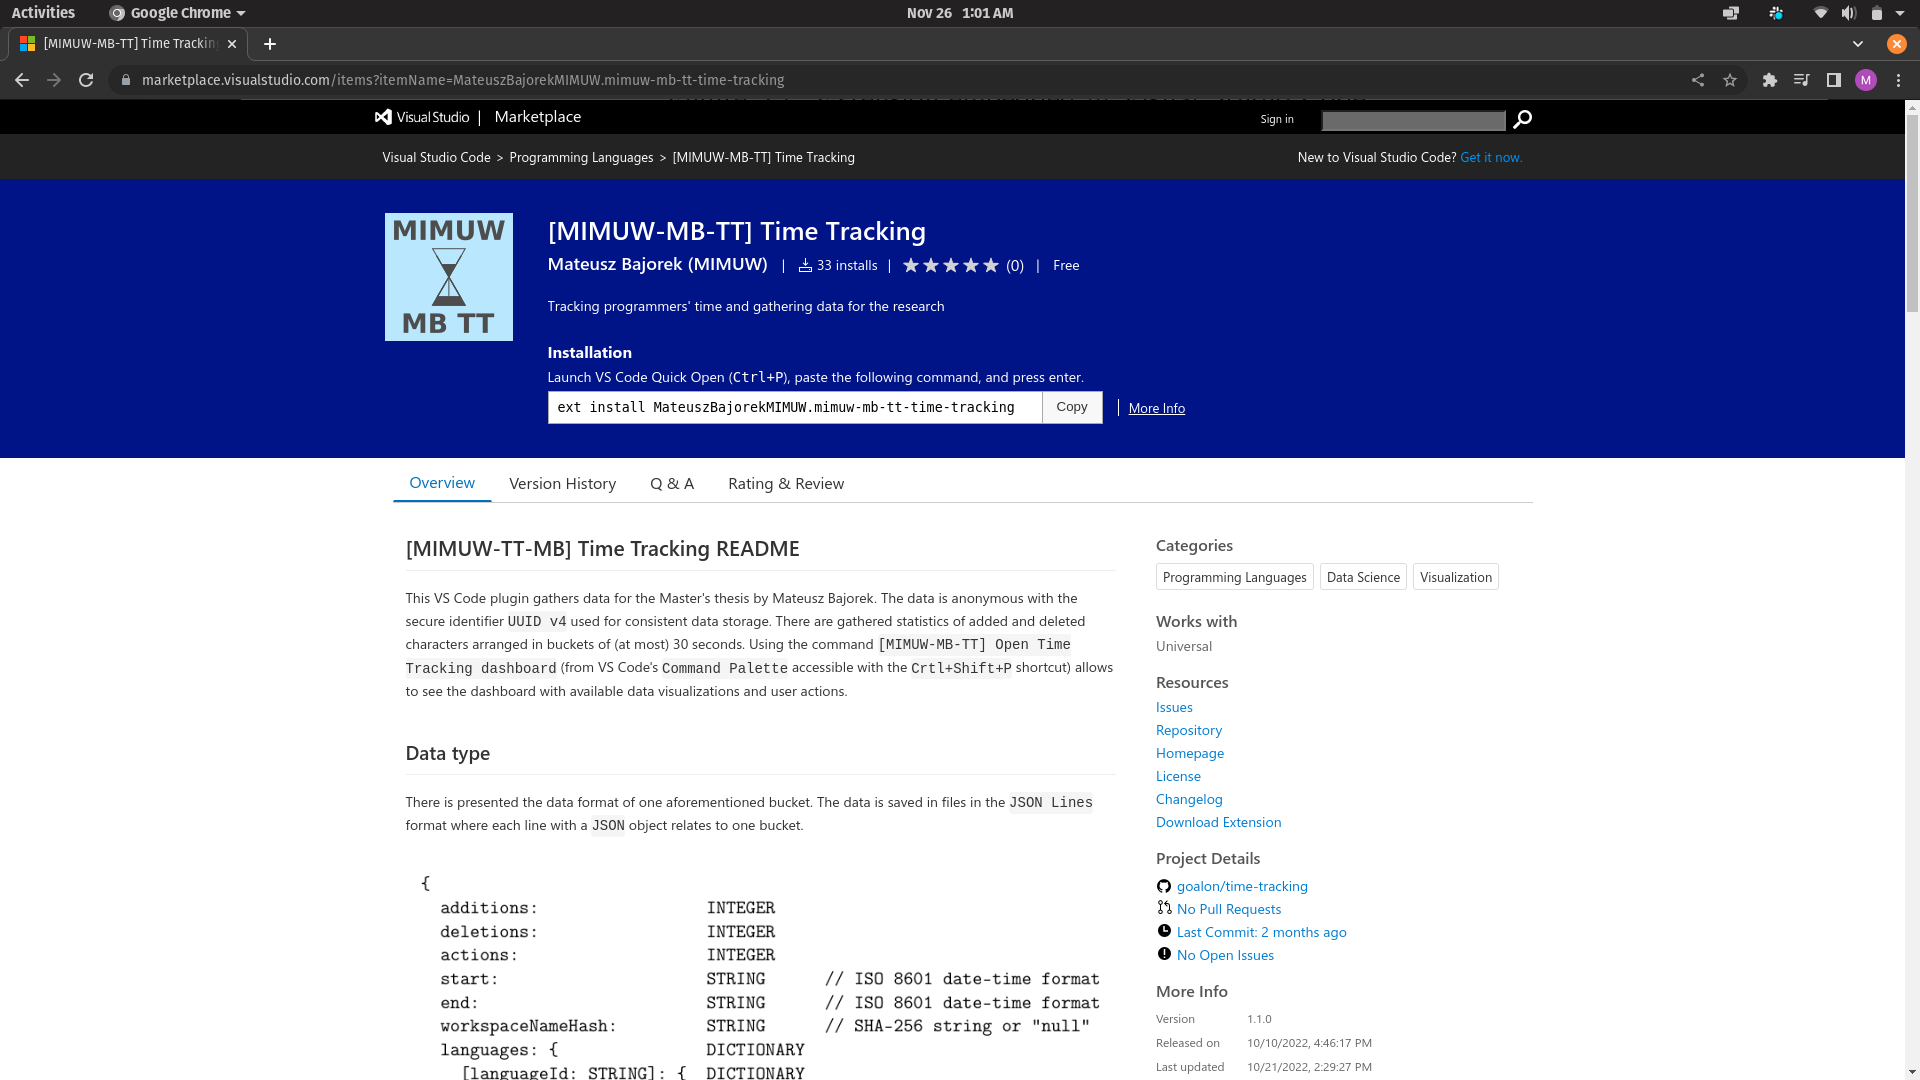
\includegraphics[scale=0.22]{chapters/availability/graphics/marketplace.png}
  \caption{\textit{MIMUW-MB-TT} plugin in the VS Marketplace (as of 26 Nov 2022)}
  \label{fig:marketplace}
\end{figure}

% Mention differential privacy in open data potentially in the future. Mention the de-anonymization paper as well.

% Mention GDPR later.

% name the plugin somehow
